\subsection{Wykorzystanie głębokich sieci neuronowych do zadania klasyfikacji obrazów}

\subsubsection{Informacje Ogólne}

W ostatnich latach nastąpił dynamiczny rozwój głębokich sieci neuronowych – dużych modeli, które wyewoluowały z klasycznych sieci neuronowych. Algorytmy uzyskują bardzo wysokie wyniki w wielu zadaniach takich jak: rozpoznawanie obrazu, rozpoznawanie mowy, analiza tekstu pisanego, synteza mowy. Zaletą głębokich sieci neuronowych do zadania klasyfikacji obrazów jest możliwość automatycznej ekstrakcji cech, w przeciwieństwie do klasycznych algorytmów rozpoznawania obrazu, których dobór wymaga wiedzy eksperckiej bazującej na tzw. inżynierii cech. Dzięki tej umiejętności, głębokie sieci neuronowe są w stanie wyodrębnić z badanego obrazu istotne cechy, które mają największy wpływ na możliwości klasyfikacji. 

\subsubsection{Konwolucyjne sieci neuronowe}

Odmianą głębokich sieci neuronowych służącą do analizy obrazu są splotowe (konwolucyjne) sieci neuronowe. Typowa splotowa sieć neuronowa składa się z kombinacji 3 podstawowych typów warstw: 
\begin{itemize}	
	\item warstwa splotowa(konwolucyjna), 
	\item warstwa redukująca rozmiar (pooling). 
	\item warstwa aktywacji \\
\end{itemize}	

Dodatkowo wykorzystuję się klasyczne warstwy neuronowe tzw. warstwy pełnego połączenia. Splotowa sieć neuronowa przyjmuje na wejście obraz, który następnie jest przetwarzany przez kolejne warstwy. Warstwa splotowa wykonuje wielokrotnie operację splotu dyskretnego na obrazie wejściowym tworząc na wyjściu mapy cech. Operacja splotu dyskretnego w obszarach analizy obrazu wykorzystywana jest do filtracji. Następnie, przefiltrowane obrazy trafiają na nieliniową funkcję aktywacji, która przetwarza każdy piksel. Dodatkowo, po niektórych warstwach aktywacji umieszczona jest warstwa redukująca rozmiar, która zmniejsza liczbę pikseli w przetwarzanych obrazach. Wyjście ostatniej warstwy splotowej trafia na klasyczną sieć neuronową. \\

Uczenie klasycznych sieci neuronowych z dużą liczbą warstw jest bardzo trudne, często niemożliwe. W głębokich sieciach neuronowych wprowadzono szereg modyfikacji, które umożliwiły efektywny trening tak dużych modeli. Warstwy splotowe można interpretować jako zbiór neuronów połączonych z niewielką ilością neuronów w warstwie poprzedzającej, w przeciwieństwie do warstw klasycznych gdzie neuron połączony jest ze wszystkimi neuronami w poprzedniej warstwie. Ponadto, neurony posiadają grupowo współdzielone wagi (w ramach jednego filtru splotowego). Wymienione właściwości umożliwiają znaczną redukcję ilości parametrów, co umożliwia skuteczne uczenie takich struktur. Ponadto, szeroko stosowana funkcja aktywacji ReLU redukuje problem znikającego gradientu, ze względu na niemożliwość nasycenia się funkcji, jak ma to miejsce w klasycznych funkcjach aktywacji (funkcja sigmoidalna czy tangens hiperboliczny). \\

Cechą odróżniającą głębokie sieci neuronowe od klasycznych systemów klasyfikacji obrazów jest możliwość automatycznej ekstrakcji cech. Poprawna ekstrakcja cech jest kluczowym elementem każdego systemu klasyfikacji. Warstwy splotowe działają jako ekstraktor cech, które następnie podawane są na klasyczny klasyfikator neuronowy. W przypadku klasycznych systemów algorytmy ekstrakcji cech i ich parametry dobierane są przez badacza.

\subsubsection{Przykład}

\begin{itemize}
	\item Klasyczna sieć neuronowa rozpoznająca cyfry:
		\begin{figure}[H]
			\centering
			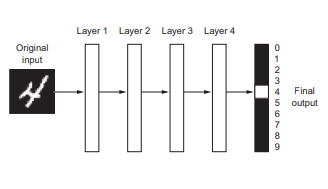
\includegraphics[width=0.5\linewidth]{S3_1.png}
			\caption{Krzywa ROC}
		\end{figure}
	\item Głęboka sieć konwolucyjna rozpoznająca cyfry:
		\begin{figure}[H]
			\centering
			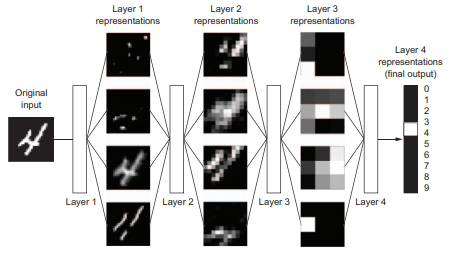
\includegraphics[width=0.5\linewidth]{S3_2.png}
			\caption{Krzywa ROC}
		\end{figure}
\end{itemize}

\subsubsection{Przykładowe architektury}

\begin{itemize}
	\item LeNet(1990)
	\item AlexNet(2012)
	\item VGGNet(2014)
	\item ResNet(2015)
\end{itemize}
